\documentclass[a4paper]{article}
\usepackage[left=2.1cm, right=2.1cm, top=2.1cm]{geometry}
\usepackage{lipsum}
\usepackage{tikzpagenodes}
\usepackage{pgfplots}
\usepackage{tikz}
\usepackage{tikz-3dplot}
\usetikzlibrary{arrows,decorations.pathmorphing,backgrounds,positioning,fit,matrix}
\pgfplotsset{compat=1.8}
\usepackage{graphics} % for pdf, bitmapped graphics files
\usepackage{epsfig} % for postscript graphics files
\usepackage[colorlinks=true,citecolor=green]{hyperref}
\usepackage{cite}
\usepackage{amsmath,amssymb,amsfonts}
\usepackage{algorithmic}
\usepackage{graphicx}
\usepackage{url}
\usepackage{cite}
\usepackage{bm}
\usepackage{pbox}
\usepackage{siunitx,booktabs,etoolbox}
\usepackage{ulem}
\usepackage[framed,numbered,autolinebreaks,useliterate]{mcode}
\usepackage{filecontents}
%\usepackage{bigfoot} % to allow verbatim in footnote


\def\BibTeX{{\rm B\kern-.05em{\sc i\kern-.025em b}\kern-.08em
    T\kern-.1667em\lower.7ex\hbox{E}\kern-.125emX}}


\begin{document}

\title{Exercise on SIFT \& KD-tree based feature matching}
\author{xiahaa@space.dtu.dk}
\maketitle%%

In this exercise, you will work on SIFT and KD-tree based feature matching.

\section{SIFT}
\begin{enumerate}
\item Learn how to use the VLFeat (\textbf{src/3rdparty/vlfeat-0.9.21}), google VLFeat, learn how to setup.
\item Find on \url{http://www.vlfeat.org/overview/sift.html} about how to use VLFeat for SIFT feature detection and matching.
\item Find on \url{http://www.vlfeat.org/overview/kdtree.html} about how to use KD tree in VLFeat and create a matcher by using the KD tree.
\end{enumerate}

\textbf{It is a good idea to organize your code as separate functions which can be reused.}

\begin{figure*}[!b]
\centering
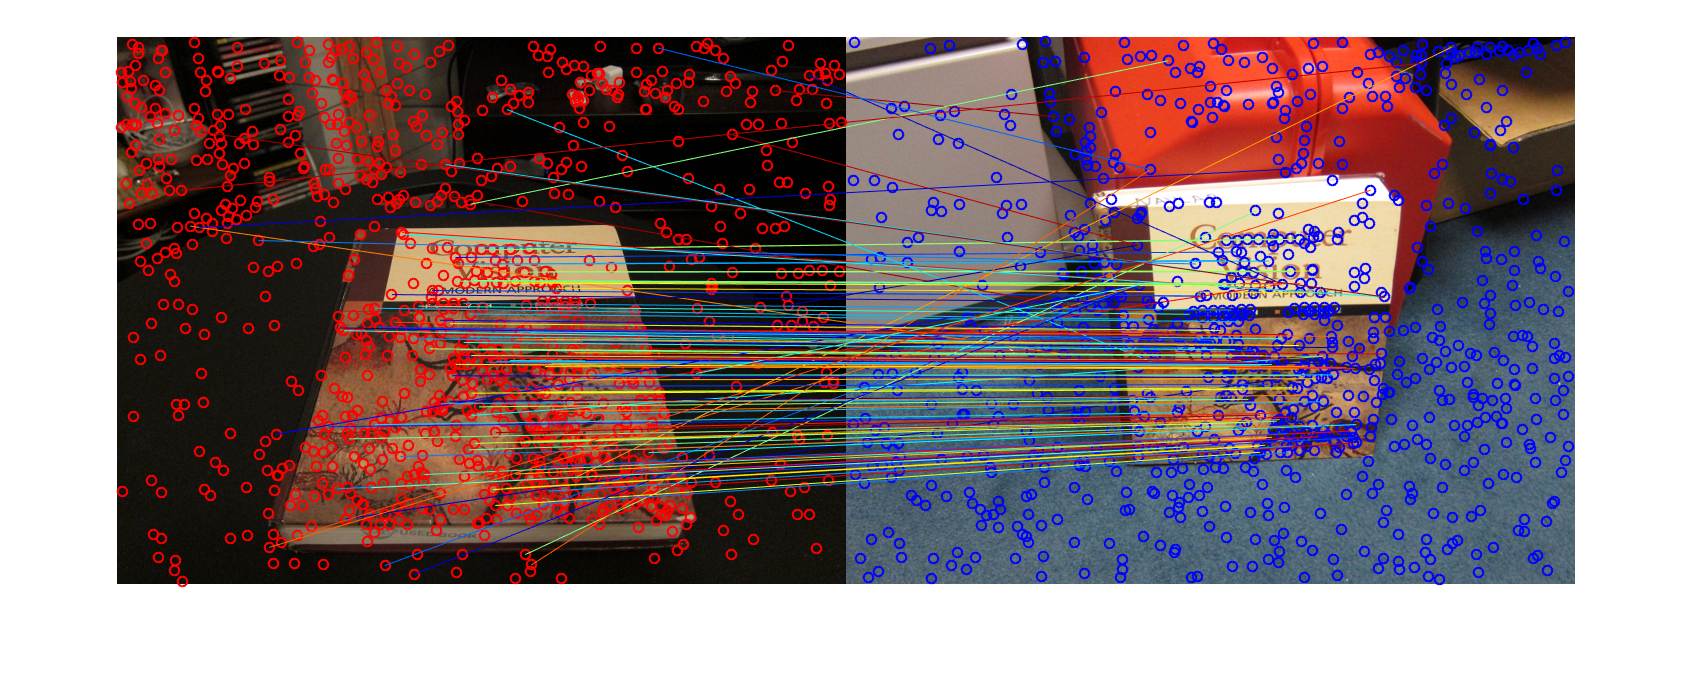
\includegraphics[scale=0.3]{figures/sift.png}
\caption{Example of SIFT matching result.}
\end{figure*}

\end{document}